\chapter{NOOSFERO}

O Noosfero é uma plataforma \textit{open source} para a construção de redes sociais
e colaborativas. Desenvolvido em Ruby on Rails e licenciado sob AGPL versão 3, o
projeto ainda conta com desenvolvimento ativo.

Além dos mecanismos de interação social, o Noosfero também conta com um sistema de
gerenciamento de conteúdo, o que possibilita a criação de \textit{blogs} e o
compartilhamento de arquivos. A plataforma também pode ser estendida por
\textit{plugins} desenvolvidos pela comunidade, e conta com o conceito de
\textit{environments}, que permitem a criação de diversas redes isoladas funcionando
sobre uma mesma instância da aplicação.

\begin{figure}[h]
	\centering
		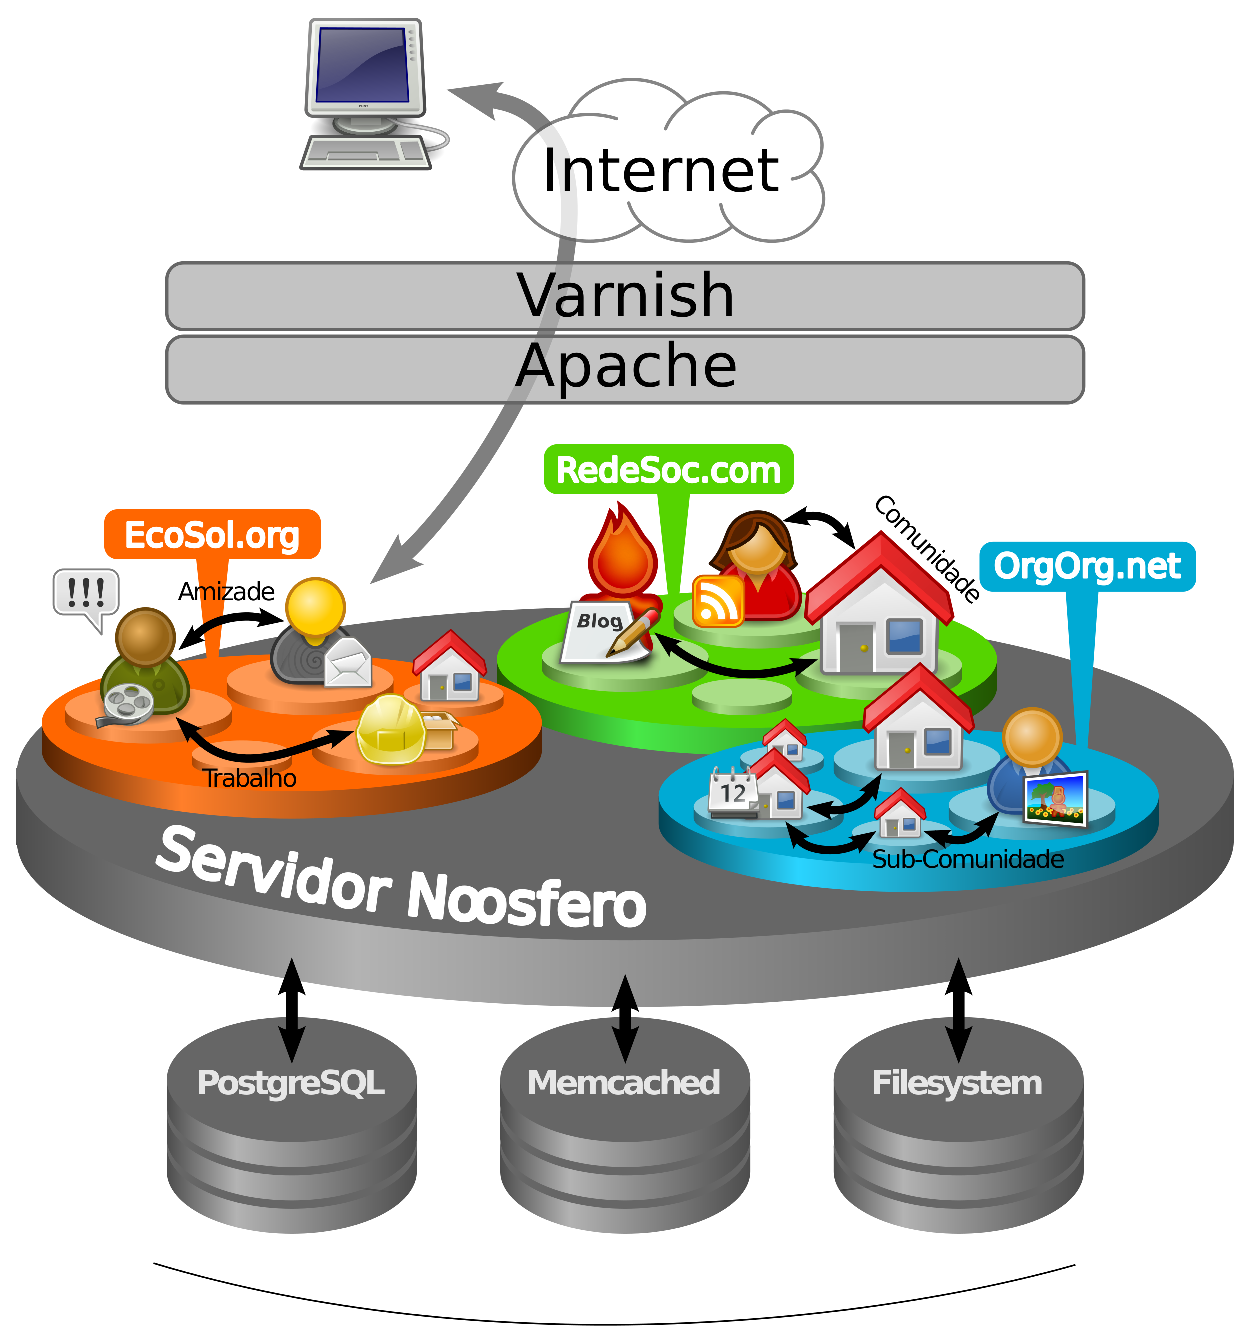
\includegraphics[keepaspectratio=true,scale=0.4]{figuras/noosfero_estrutura.eps}
	\caption{Arquitetura do Noosfero}
	\label{fig:noosferoEstrutura}
\end{figure}
% adicionar fonte

As informações e publicações de pessoas e organizações podem ser públicas ou
privadas. Já os relacionamentos entre estas entidades podem ser tanto simétricos
como assimétricos.

Enquanto um relacionamento simétrico depende da concordância de ambas as partes para
o compartilhamento das informações privadas (como por exemplo amizades ou
filiações), um relacionamento assimétrico depende apenas do interesse de uma das
entidades em acompanhar as informações públicas de algum perfil (como no caso da
funcionalidade de seguidores).



\section{INICIATIVA DE FEDERAÇÃO}

% como e por que motivo a iniciativa foi tomada


\subsection{Acordo com especificações existentes}

% problema em conciliar os conceitos
% diferença nos relacionamentos com o Diaspora


\subsection{Definições}

% projeto
% o que a federação com outras redes deve cobrir

